%% This Beamer template is based on the one found here: https://github.com/sanhacheong/stanford-beamer-presentation, and edited to be used for Stanford ARM Lab

\documentclass[10pt]{beamer}
%\mode<presentation>{}

\usepackage{media9}
\usepackage{amssymb,amsmath,amsthm,enumerate}
\usepackage[utf8]{inputenc}
\usepackage{array}
\usepackage[parfill]{parskip}
\usepackage{graphicx,animate}
\usepackage{caption}
\usepackage{subcaption}
\usepackage{bm}
\usepackage{amsfonts,amscd}
\usepackage[]{units}
\usepackage{listings}
\usepackage{multicol}
\usepackage{multirow}
\usepackage{tcolorbox}
\usepackage{physics}
\usepackage{movie15}
% Enable colored hyperlinks
\hypersetup{colorlinks=true}

% The following three lines are for crossmarks & checkmarks
\usepackage{pifont}% http://ctan.org/pkg/pifont
\newcommand{\cmark}{\ding{51}}%
\newcommand{\xmark}{\ding{55}}%

% Numbered captions of tables, pictures, etc.
\setbeamertemplate{caption}[numbered]
\usepackage{media9} 
%\usepackage[superscript,biblabel]{cite}
\usepackage{algorithm2e}
\renewcommand{\thealgocf}{}

% Bibliography settings
\usepackage[style=authoryear]{biblatex}
\setbeamertemplate{bibliography item}{\insertbiblabel}

\addbibresource{bibliography.bib}

% Glossary entries
\usepackage[acronym]{glossaries}
\newacronym{ML}{ML}{machine learning}
\newacronym{HRI}{HRI}{human-robot interactions}
\newacronym{RNN}{RNN}{Recurrent Neural Network}
\newacronym{LSTM}{LSTM}{Long Short-Term Memory}


\theoremstyle{remark}
\newtheorem*{remark}{Remark}
\theoremstyle{definition}

\newcommand{\empy}[1]{{\color{darkorange}\emph{#1}}}
\newcommand{\empr}[1]{{\color{cardinalred}\emph{#1}}}
\newcommand{\examplebox}[2]{
\begin{tcolorbox}[colframe=darkcardinal,colback=boxgray,title=#1]
#2
\end{tcolorbox}}

\usetheme{Stanford} 
\def \i  {\item}
\def \ai {\item[] \quad \arrowbullet}
\newcommand \si[1]{\item[] \quad \bulletcolor{#1}}
\def \wi {\item[] \quad $\ \phantom{\Rightarrow}\ $}
\def \bi {\begin{itemize}\item}
\def \ei {\end{itemize}}
\def \be {\begin{equation*}}
\def \ee {\end{equation*}}
\def \bie {$\displaystyle{}
\def \eie {{\ }$}}
\def \bsie {\small$\displaystyle{}
\def \esie {{\ }$}\normalsize\selectfont}
\def \bse {\small\begin{equation*}}
\def \ese {\end{equation*}\normalsize}
\def \bfe {\footnotesize\begin{equation*}}
\def \efe {\end{equation*}\normalsize}
\renewcommand \le[1] {\\ \medskip \lefteqn{\hspace{1cm}#1} \medskip}
\def \bex {\begin{example}}
\def \eex {\end{example}}
\def \bfig {\begin{figure}}
\def \efig {\end{figure}}
\def \btheo {\begin{theorem}}
\def \etheo {\end{theorem}}
\def \bc {\begin{columns}}
\def \ec {\end{columns}}
\def \btab {\begin{tabbing}}
\def \etab {\end{tabbing}\svneg\svneg}
\newcommand \col[1]{\column{#1\linewidth}}
\def\vneg  {\vspace{-5mm}}
\def\lvneg {\vspace{-10mm}}
\def\svneg {\vspace{-2mm}}
\def\tvneg {\vspace{-1mm}}
\def\vpos  {\vspace{5mm}}
\def\lvpos {\vspace{10mm}}
\def\svpos {\vspace{2mm}}
\def\tvpos {\vspace{1mm}}
\def\hneg  {\hspace{-5mm}}
\def\lhneg {\hspace{-10mm}}
\def\shneg {\hspace{-2mm}}
\def\thneg {\hspace{-1mm}}
\def\hpos  {\hspace{5mm}}
\def\lhpos {\hspace{10mm}}
\def\shpos {\hspace{2mm}}

\logo{
\includegraphics[height=0.43in]{style_files_stanford/wlogo.png}}

\makeatletter
\let\@@magyar@captionfix\relax
\makeatother

\title[Conditional Random Fields]{Conditional Random Fields}


\begin{document}

\author[Shrey Satapara]{
	\begin{tabular}{c} 
	\Large
	Shrey Satapara\\
    \footnotesize AI22MTECH02003 \\
    % Author Two \\
    % \footnotesize \href{mailto:author.2@kaust.edu.sa}{author.2@kaust.edu.sa}
\end{tabular}
\vspace{-4ex}}

\institute{
	\vskip 5pt
	\begin{figure}
		\centering
			
\includegraphics[height=0.5in]{style_files_stanford/logo.png}
	\end{figure}
	\vskip 10pt
	Department of Artificial Intelligence\\
	\vskip 3pt
}

% \date{June 15, 2020}
%\date{\today}

\begin{noheadline}
\begin{frame} \maketitle \end{frame}
\end{noheadline}

\setbeamertemplate{itemize items}[default]
\setbeamertemplate{itemize subitem}[circle]

\begin{frame}{About Referred Paper}
\begin{itemize}
    \item Title: Corpus for Automatic Structuring of Legal Documents \cite{2201.13125}
    \item For segmentation of legal judgment documents in English  into topical and coherent parts. Each of these parts is annotated with a label coming from a list of pre-defined Rhetorical Roles. They proposed automatically predicting rhetorical roles using SciBERT-HSLN architecture. Which use CRF as final classification layer. \cite{2102.06008}.
    \item So here, I've explained Conditional Random Fields.
\end{itemize}
    
\end{frame}

\begin{frame}
\frametitle{Motivation for CRF: Shortcomings of Hidden Markov Model}
\begin{figure}
		\centering
			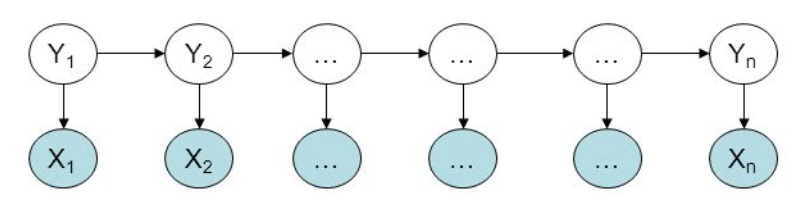
\includegraphics[height=0.8in]{style_files_stanford/hmm1.png}
	\end{figure}
	\begin{itemize}
	    \item HMM Models direct dependence between each state and only it's corresponding observation.
		\begin{itemize}
    		\item NLP Example: In sequence sentence classification task, target may not only depend on current sentence but also target label of previous sentence or previous sentence.
		\end{itemize}
		\item Mismatch between learning objective function and prediction objective function.
		\begin{itemize}
    		\item HMM learns a joint distribution of state and observation \(P(X,Y)\) but in a prediction task, we need conditional probability \(P(Y|X)\)
		\end{itemize}
	\end{itemize}
\end{frame}

\begin{frame}{Solution: Conditional Random Fields(CRF)}
\begin{itemize}
    \item To overcome the problem of HMM, CRF came into picture.
    \item  Conditional Random Fields are a type of Discriminator classifier, and as such, they model the decision boundary between the different classes.
    \item In CRFs, our input data is sequential, and we have to take previous context into account when making predictions on a data point. To model this behavior, we will use Feature Functions, that will have multiple input values, which are going to be:
    \begin{itemize}
    		\item The set of input vectors, X
            \item The position i of the data point we are predicting
            \item The label of data point i-1 in X
            \item The label of data point i in X
		\end{itemize}
	\item We define feature function as \(f(X,i,l_{i-1},l_i)\)
\end{itemize}
\end{frame}

\begin{frame}{What is feature function}
\begin{itemize}
    \item The purpose of the feature function is to express some kind of characteristic of the sequence that the data point represents. 
    \item For instance, if we are using CRFs for Parts-of-Speach tagging, than
    \begin{itemize}
        \item \(f(X, i, L_{i - 1}, L_{i} ) = 1\) if \(L_{i - 1}\) is a Noun, and \(L_{i}\)is a Verb. 0 otherwise.
        \item Similarly, \(f(X, i, L_{i - 1}, L_{i} ) = 1\) if \(L_{i - 1}\) is a Verb and \(L_{i}\) is an Adverb. 0 otherwise.
    \end{itemize}
\end{itemize}
\end{frame}

\begin{frame}{Probability Distribution for Conditional Random Fields}
\begin{itemize}
    \item Each feature function is based on previous label and current input. To build conditional field we assign each feature function some weight(lambda values) which our algorithm is going to learn.
\end{itemize}
\begin{equation}
    P(y,X,\lambda) = \frac{1}{Z(X)}exp{\Sigma_{i=1}^n\Sigma_j\lambda_jf_i(X,i,y_{i-1},y_i)}
\end{equation}
Where,
\begin{equation}
    Z(X) = \Sigma_{y'\in y} \Sigma_{i=1}^n\Sigma_j\lambda_jf_i(X,i,y_{i-1},y_i)
\end{equation}
\end{frame}

\begin{frame}{Parameters Estimation of Weights(Lambda)}
\begin{itemize}
    \item To estimate the parameters (lambda), we will use Maximum Liklihood Estimation. To apply the technique, we will first take the Negative Log of the distribution, to make the partial derivative easier to calculate:
\end{itemize}
\begin{align*}
    L(y,X,\lambda) &= -log(\Pi_{k=1}^mP(y^k|x^k,\lambda))\\
    &= -\Sigma_{k=1}^mlog[\frac{1}{Z(X_m)}exp{\Sigma_{i=1}^n\Sigma_j\lambda_jf_i(X,i,y_{i-1},y_i)}]
\end{align*}
\begin{center}
    Negative Log Liklihood of the CRF Probability Distribution
\end{center}
\end{frame}
\begin{frame}{Parameters Estimation of Weights(contd.)}
    \begin{itemize}
        \item To apply Maximum Liklihood on the Negative Log function, we will take the argmin (because minimizing the negative will yield the maximum). To find the minimum, we can take the partial derivative with respect to lambda, and get:
    \end{itemize}
\begin{equation}
    \partial L(X,y,\lambda) = \frac{-1}{m}\Sigma_{k=1}^mF_j(y^k,x^k) + \Sigma_{k=1}^m p(y|x^k,\lambda)F_j(y,x^k)
\end{equation}
where,
\begin{equation}
    F_j(y,x) = \Sigma_{i=1}^nf_i(X,i,y_{i-1},y_i)
\end{equation}
\begin{center}
    Partial Derivative w.r.t. lambda
\end{center}
\end{frame}
\begin{frame}{Learning of Weights using Gradient Decent Algorithm}
\begin{itemize}
    \item We use the Partial Derivative as a step in Gradient Descent. Gradient Descent updates parameter values iteratively, with a small step, until the values converge. Our final Gradient Descent update equation for CRF is:
\end{itemize}
    \begin{equation}
        \lambda = \lambda - \alpha[\Sigma_{k=1}^mF_j(y^k,x^k) + \Sigma_{k=1}^m p(y|x^k,\lambda)F_j(y,x^k)]
    \end{equation}
where, \(\alpha\) is learning rate
\end{frame}
\begin{frame}{Applications of CRF}
\nocite{}
\begin{itemize}
    \item Given their ability to model sequential data, CRFs are often used in Natural Language Processing, and have many applications in that area.
    \item One such application we discussed is Parts-of-Speech tagging. Parts of speech of a sentence rely on previous words, and by using feature functions that take advantage of this, we can use CRFs to learn how to distinguish which words of a sentence correspond to which POS
    \item Another similar application is Named Entity recognition, or extracting Proper nouns from sentences.
    \item Other applications include parts-recognition in Images and gene prediction.
\end{itemize}
\end{frame}
\begin{frame}[allowframebreaks]{References}
\printbibliography
\end{frame}
\begin{frame}{}
    \textsc{\huge THANK YOU}
\end{frame}
\end{document}